\documentclass[a4paper,11pt]{article}

\usepackage[utf8]{inputenc}
\usepackage[T1]{fontenc}
\usepackage[margin=2.5cm]{geometry}
\usepackage{amsmath}
\usepackage{graphicx}
\usepackage{booktabs}
\usepackage{xcolor}
\usepackage{subcaption}
\usepackage[hidelinks]{hyperref}
\usepackage[sc]{titlesec}

\newcommand{\todo}[1]{\textcolor{red}{[TODO: #1]}}
\newcommand{\kernel}[1]{\texttt{#1}}
\newcommand{\GBs}{\,GB/s}
\newcommand{\GFs}{\,GFLOP/s}

\title{\Large{\sc{Performance Engineering}}\\[2mm]
  Performance Analysis and Modelling of the CloverLeaf Mini-App\\
  on the HAICGU Kunpeng~920 Cluster}
\author{Jort Oosterveld S5545781 \& Sergiu-Adrian Preda S6778542 \\ Group 11}
\date{Draft, \today}

\begin{document}
\setlength\parindent{0pt}
\setlength{\parskip}{0.6em}
\maketitle

\begin{abstract}
We analyse and model the C kernels of the CloverLeaf reference mini-app on a dual-socket Kunpeng~920 node
(128 cores, 4 NUMA domains).
Internal timers, PAPI counters per kernel, Linux \texttt{perf} and the DDR-controller counters show that the
code is memory-bound everywhere: its arithmetic intensity (0.2\,flop/B) is 25$\times$ below the ridge point
of the measured roofline (5\,flop/B).
The default pure-OpenMP configuration reaches less than half (48\%) of the best STREAM bandwidth, because
transparent huge pages place the application's arrays unevenly on the NUMA domains.
Disabling huge pages for the process, without touching the source, gives a 1.7$\times$ speed-up and
79\% of the best STREAM bandwidth.
An analytic model of the kernels predicts the measured DRAM traffic within 1--5\%, and identifies
the remaining optimisation potential as a reduction of the bytes moved.
\end{abstract}

% =============================================================================
\section{Introduction}
% =============================================================================
CloverLeaf is a mini-app that solves the compressible Euler equations on a two-dimensional structured
grid with an explicit second-order Lagrangian--Eulerian scheme~\cite{mallinson2013}.
It is a typical stencil code, and a popular case study for memory-bound performance
engineering~\cite{laukemann2023}.
We work on the reference implementation (\texttt{CloverLeaf\_ref}, commit \texttt{b5e598d}, hybrid
MPI+OpenMP) and restrict ourselves to its \emph{C kernels}, which are selected at run time with
\texttt{use\_c\_kernels} in the input deck.
The Fortran code outside the kernels (driver, input, halo-exchange bookkeeping) is unchanged and is not
optimised.
The target is one standard compute node of the HAICGU cluster.

The report follows the structure of the assignment.
Section~\ref{sec:app} describes the application and the test problems, Section~\ref{sec:system} the system and
the tool chain, and Section~\ref{sec:method} the measurement methodology, including how we checked that the
tools themselves are correct.
Section~\ref{sec:analysis} presents the performance analysis (where does the time go?),
Section~\ref{sec:model} the performance model (what is attainable?), and Section~\ref{sec:opt} the
optimisation plan that follows from both.

% =============================================================================
\section{Application and test problems}
\label{sec:app}
% =============================================================================
One time step executes, in this order, the kernels listed in Table~\ref{tab:kernels}:
the equation of state (\kernel{ideal\_gas}), artificial viscosity, the stable time step
(\kernel{calc\_dt}), a predictor and a corrector pressure--volume work step (\kernel{pdv}), the
acceleration of the nodes, the volume fluxes, the advection of cell quantities (\kernel{advec\_cell})
and of momentum (\kernel{advec\_mom}) in two sweeps, and the reset of the time levels.
Every kernel is a loop nest over the 2D grid with a stencil of at most $\pm1$ cell, and
\kernel{advec\_cell} and \kernel{advec\_mom} contain an upwind/limiter loop with data-dependent indices.

All 2D fields are double-precision arrays of $(n_x+5)\times(n_y+5)$ elements.
We use two problem sizes, both with 87 time steps and the built-in quality check (\texttt{test\_problem~4}
resp.\ \texttt{2}), which compares the final kinetic energy with a reference value:
\begin{itemize}
  \item \textbf{bm3840}: $3840^2$ cells = 14.7\,M cells.
        About 25 arrays of 118\,MB each, i.e.\ a working set of $\approx$3\,GB, far beyond all caches
        (2$\times$64\,MB L3). This is our main problem.
  \item \textbf{bm960}: $960^2$ cells, 0.2\,GB; it partly fits in the L3 and is used to see how
        synchronisation costs show up at small sizes.
\end{itemize}
Every run reported here printed \texttt{PASSED}.

% =============================================================================
\section{Target system and tool chain}
\label{sec:system}
% =============================================================================
\begin{itemize}
  \item \textbf{Node:} HAICGU standard compute node, 2$\times$ Kunpeng~920 (ARMv8, 64 cores each,
        2.6\,GHz), 4 NUMA domains of 32 cores, 16 channels of DDR4-2666 (128\,GB, theoretical
        341\GBs{}). We use whole nodes exclusively (\texttt{--exclusive}) in the \texttt{cn-ib} partition.
  \item \textbf{Operating system:} a RHEL-8-compatible Linux on aarch64 with 64\,KB base pages; transparent huge pages
        (THP) are set to \texttt{always} and the huge-page size is 512\,MB.
  \item \textbf{Software:} GCC and GFortran 14.1.0, OpenMPI 5.0.3, PAPI 7.1.0 (site module), Linux
        \texttt{perf}. Flags: \texttt{-O3 -march=native -funroll-loops -fopenmp} (the project's \texttt{GNU}
        settings) plus \texttt{-g}, which does not change the generated code.
  \item \textbf{Placement:} \texttt{OMP\_PLACES=cores}, \texttt{OMP\_PROC\_BIND=close}; for MPI runs one rank
        per NUMA domain (4$\times$32) or per socket (2$\times$64), bound to cores.
\end{itemize}
A configuration is written ``$r\times t$'' for $r$ MPI ranks with $t$ OpenMP threads each.

% =============================================================================
\section{Methodology}
\label{sec:method}
% =============================================================================
\subsection{Measurement tools}
We use three independent sources, as required by the assignment.

\textbf{(1) CloverLeaf's internal profiler} (\texttt{profiler\_on}) reports the wall-clock time of each
algorithmic phase from \texttt{gettimeofday}. It gives the overview and the scaling studies.

\textbf{(2) PAPI, per kernel.}
We added a small instrumentation layer (\texttt{papi\_prof}) that wraps the \texttt{omp parallel} region of
each C kernel. Every thread keeps its own event set running and reads the counters at region entry and exit;
the results are written per thread at process exit. The macros compile to nothing without
\texttt{-DUSE\_PAPI}. Because the PMU has few counters, events are measured in separate runs:
cycles+instructions, L1D/L2 accesses and misses, an instruction-mix set (loads, stores, FP, SIMD), and a set with
back-end/front-end stall cycles and bus accesses.

\textbf{(3) Linux \texttt{perf}.} \texttt{perf record} (sampling, 999\,Hz) attributes cycles to functions;
\texttt{perf stat} gives whole-run counters; and the HiSilicon DDR-controller PMU
(\texttt{hisi\_sccl*\_ddrc*/flux\_rd,wr}) is read system-wide and measures the bytes that really cross the
memory interface, per memory controller.

\subsection{Protocol}
Each configuration is run three times and we report the median (min--max where relevant). The timed region is
the complete run of 87 steps, including start-up.

\subsection{Checks of the tools}
\label{sec:checks}
\begin{itemize}
  \item \emph{Correctness of the code under instrumentation:} all runs, with and without PAPI, pass the quality check.
  \item \emph{Overhead:} the PAPI build needs 521--523\,s on one core against 528\,s for the plain build, i.e.\ no
        measurable overhead; at 128 threads the difference is inside the run-to-run noise.
  \item \emph{Timers vs.\ PAPI:} the per-kernel PAPI times add up to 523\,s on one core (wall clock of that run:
        522\,s), and the kernel shares agree with the internal profiler within one percentage point
        (e.g.\ \kernel{advec\_mom} 28.5\% vs.\ 28.1\%).
  \item \emph{Counters vs.\ counters:} \texttt{MEM\_ACCESS} equals \texttt{PAPI\_L1\_DCA}, and
        loads$+$stores equal L1D accesses, in every kernel. The cycle counter gives 2.59\,GHz on one core.
  \item \emph{Memory counters vs.\ a known byte count:} STREAM moves a known number of bytes. Its DDR-controller
        total (7.43\,G counts) matches the expected traffic with write-allocate if one count is 32\,B
        (238\,GB vs.\ 234\,GB, 2\% difference; 224\,GB for the timed loops alone plus initialisation and
        result check); we use this unit throughout.
\end{itemize}

% =============================================================================
\section{Performance analysis}
\label{sec:analysis}
% =============================================================================
\subsection{Where the time goes}
Table~\ref{tab:kernels} shows the time share of every kernel and the hardware metrics measured with PAPI.
On one core the run is dominated by the two advection kernels (48\%), followed by the two PdV
passes (18\%) and \kernel{calc\_dt} (12\%). With 128 cores \kernel{advec\_mom} grows to 44\% of the time
because it scales worst of the large kernels (14$\times$, against 22--59$\times$ for the others), while \kernel{calc\_dt},
\kernel{viscosity} and \kernel{ideal\_gas}, which are compute-heavy on one core, shrink to about 12\% together.

\begin{table}[t]
  \centering\small
  \begin{tabular}{rlrrrrrr}
\toprule
\# & kernel & \multicolumn{2}{c}{time share (\%)} & IPC & vector & FP scalar & back-end \\
 & & 1 core & 128 cores & 1 core & ins.\ (\%) & ins.\ (\%) & stall (\%) \\
\midrule
1 & \texttt{advec\_mom} & 28.6 & 44.0 & 0.85 & 16 & 17 & 71 / 94 \\
2 & \texttt{advec\_cell} & 19.4 & 19.4 & 0.75 & 12 & 25 & 73 / 93 \\
3 & \texttt{calc\_dt} & 11.8 & 4.8 & 0.65 & 0 & 64 & 75 / 84 \\
4 & \texttt{pdv\_correct} & 9.0 & 5.0 & 0.35 & 62 & 0 & 83 / 93 \\
5 & \texttt{pdv\_predict} & 8.6 & 4.6 & 0.35 & 60 & 0 & 87 / 95 \\
6 & \texttt{ideal\_gas} & 7.4 & 4.7 & 0.52 & 0 & 53 & 79 / 92 \\
7 & \texttt{viscosity} & 5.7 & 2.2 & 1.06 & 0 & 64 & 60 / 79 \\
8 & \texttt{accelerate} & 5.2 & 4.1 & 0.63 & 41 & 0 & 77 / 93 \\
9 & \texttt{flux\_calc} & 2.2 & 3.0 & 0.53 & 45 & 0 & 80 / 96 \\
10 & \texttt{reset\_field} & 1.1 & 3.2 & 0.56 & 0 & 0 & 80 / 97 \\
11 & \texttt{revert} & 0.5 & 1.3 & 0.64 & 0 & 0 & 78 / 96 \\
12 & \texttt{field\_summary} & 0.4 & 0.2 & 0.64 & 56 & 24 & 72 / 90 \\
13 & \texttt{update\_halo} & 0.1 & 3.5 & 0.67 & 3 & 0 & 49 / 95 \\
\bottomrule
\end{tabular}

  \caption{Per-kernel time share (bm3840, 87 steps; ``128 cores'' = 1x128 with the default THP setting),
    IPC, share of SIMD and scalar floating-point instructions among all instructions, and back-end stall
    cycles as a share of cycles on 1 / 128 cores. Numbers refer to Figure~\ref{fig:roofline}.
    \kernel{reset\_field}, \kernel{revert} and \kernel{update\_halo} do no floating-point work.}
  \label{tab:kernels}
\end{table}

\subsection{Hardware counters: the kernels are latency- and memory-bound}
On one core the IPC is only 0.35--1.07, and 60--87\% of all cycles are back-end stalls. At 128 cores the
stall share rises to 79--97\% and the IPC falls to 0.09--0.54 (0.19 for the whole run according to
\texttt{perf stat}): the cores wait for memory.
The instruction mix shows three groups of kernels:
\begin{itemize}
  \item \kernel{pdv}, \kernel{accelerate} and \kernel{flux\_calc} are auto-vectorised
        (41--62\% NEON instructions);
  \item \kernel{calc\_dt}, \kernel{ideal\_gas} and \kernel{viscosity} execute no vector instructions at all
        (53--64\% of their instructions are scalar FP). They contain \texttt{sqrt}, which GCC does not vectorise
        without \texttt{-fno-math-errno};
  \item \kernel{advec\_mom} and \kernel{advec\_cell} are only 12--16\% vector instructions: the upwind loop
        has data-dependent indices and runs scalar.
\end{itemize}
The three scalar kernels use only 2--3\GBs{} of the 15\GBs{} that one core can sustain, so on a single core they
are limited by the latency of divisions and square roots rather than by memory.
At full node size this group is only about 12\% of the run, so it is a secondary target.

\subsection{Profile and synchronisation}
The \texttt{perf record} profile of the 128-thread run (5.8$\cdot10^{12}$ cycles) agrees with PAPI:
\kernel{advec\_mom} 35\%, \kernel{advec\_cell} 18\%, \kernel{pdv} 10.5\%, \kernel{calc\_dt} 4.6\%.
In addition it shows that \textbf{12.5\% of all cycles are spent in the OpenMP barrier}
(\texttt{gomp\_team\_barrier\_wait\_end}). The kernels consist of several consecutive worksharing loops,
each with an implicit barrier, so this is a direct optimisation target. At the small size (bm960) the
synchronisation cost dominates: 1x128 is slower than 1x64, and the halo-exchange phases take 50\% of the time.

\subsection{Scaling and the effect of memory placement}
Table~\ref{tab:configs} and Figure~\ref{fig:scaling} show the strong scaling of bm3840.
With one rank, 128 threads give a speed-up of 21 and a run-to-run spread of 21--27\,s, which is much worse
than the 4$\times$32 hybrid configuration (13.0\,s, speed-up 41, spread $<$3\%) on the same cores.

\begin{table}[t]
  \centering\small
  \begin{tabular}{lrrrr}
\toprule
configuration & cores & wall (s) & min--max (s) & speed-up \\
\midrule
1 rank $\times$ 1 thr. & 1 & 528.0 & 527.7--529.2 & 1.0 \\
1 rank $\times$ 2 thr. & 2 & 278.6 & 278.1--278.7 & 1.9 \\
1 rank $\times$ 4 thr. & 4 & 165.4 & 165.4--166.5 & 3.2 \\
1 rank $\times$ 8 thr. & 8 & 94.5 & 94.3--94.7 & 5.6 \\
1 rank $\times$ 16 thr. & 16 & 63.3 & 63.3--63.6 & 8.3 \\
1 rank $\times$ 32 thr. & 32 & 50.0 & 49.8--50.1 & 10.6 \\
1 rank $\times$ 64 thr. & 64 & 34.5 & 33.2--34.5 & 15.3 \\
1 rank $\times$ 128 thr. & 128 & 24.8 & 21.1--27.4 & 21.3 \\
2 ranks $\times$ 64 thr. & 128 & 17.1 & 15.4--20.4 & 30.9 \\
4 ranks $\times$ 32 thr. & 128 & 13.0 & 12.9--13.2 & 40.6 \\
\midrule
1 rank $\times$ 128 thr., THP off & 128 & 13.5 & 13.4--13.5 & 39.1 \\
\bottomrule
\end{tabular}

  \caption{Strong scaling of bm3840 (median of 3 runs). The last row is the same code with transparent huge
    pages disabled for the process (Section~\ref{sec:thp}).}
  \label{tab:configs}
\end{table}

\begin{figure}[t]
  \centering
  \begin{subfigure}[t]{0.49\linewidth}
    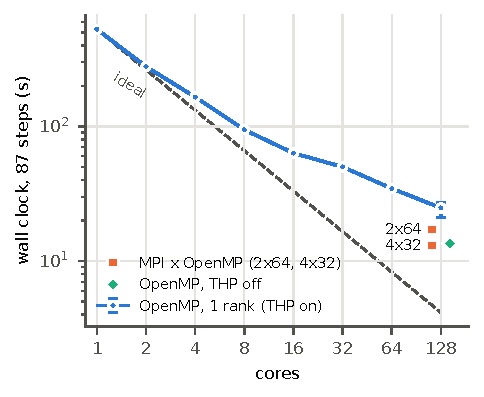
\includegraphics[width=\linewidth]{figures/fig_scaling.pdf}
    \caption{Strong scaling, bm3840.}
    \label{fig:scaling}
  \end{subfigure}\hfill
  \begin{subfigure}[t]{0.49\linewidth}
    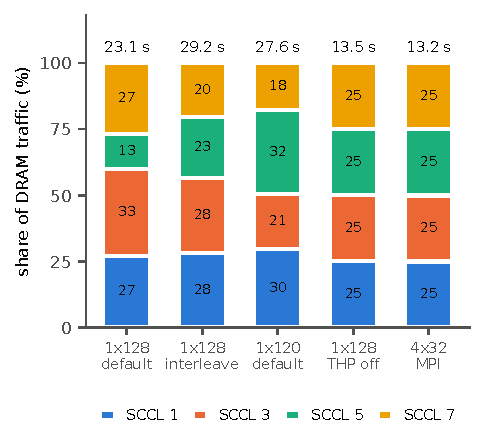
\includegraphics[width=\linewidth]{figures/fig_placement.pdf}
    \caption{DRAM traffic per controller group.}
    \label{fig:placement}
  \end{subfigure}
  \caption{(a) Wall clock against core count; error bars are min--max. (b) Share of the node's DRAM traffic
    handled by each of the four memory-controller groups (SCCL, one per NUMA domain, four DDR channels
    each), with the wall clock on top; a balanced run gives 25\% each.}
  \label{fig:scaling_placement}
\end{figure}

\subsection{Cause: transparent huge pages unbalance the memory controllers}
\label{sec:thp}
The DDR-controller counters (Figure~\ref{fig:placement}, Table~\ref{tab:placement}) explain the gap.
All variants move the same amount of data (2.8--3.0\,TB), but in the default 1$\times$128 run the busiest
controller group carries up to 1.45$\times$ the average, and the distribution differs from run to run
(e.g.\ 22/28/14/36\% and 27/33/13/27\%), while the 4$\times$32 run is perfectly balanced.
The system uses 64\,KB base pages with THP set to \texttt{always}, so a first touch allocates a
\emph{512\,MB} huge page entirely on the touching thread's NUMA domain. CloverLeaf's roughly 25 arrays
of 118\,MB are allocated back to back and occupy only about six such pages, so each page---and with it several
arrays---sits on a single domain, wherever its first-touching thread happened to run. In the 4$\times$32
configuration every rank holds only a quarter of the data and touches it from its own domain, so the problem
does not arise.

We tested the hypothesis with a small launcher that disables THP for the process tree only
(\texttt{prctl(PR\_SET\_THP\_DISABLE)}, no root needed). With THP off the 1$\times$128 run becomes perfectly
balanced and reaches the time of the MPI version (13.5\,s against 23.1\,s default, 1.71$\times$ faster),
with a spread below 1\%. Interleaving all pages (\texttt{numactl --interleave=all}) balances the controllers
but is \emph{slower} (29\,s), because three quarters of the accesses become remote; leaving eight cores idle
does not help either. Locality \emph{and} balance are needed, which first touch provides once pages are small.

\begin{table}[t]
  \centering\small
  \begin{tabular}{llrrrr}
\toprule
variant & wall (s) & DRAM (TB) & busiest/mean & bandwidth & vs.\ STREAM \\
 & median (min--max) & & controller & (GB/s) & best (\%) \\
\midrule
1x128 default & 23.1 (21.7--24.4) & 2.94 & 1.32 & 127 & 48 \\
1x128 interleave=all & 29.2 (28.3--29.5) & 3.01 & 1.13 & 103 & 39 \\
1x120 default & 27.6 (22.8--29.0) & 2.97 & 1.26 & 107 & 40 \\
1x128 THP off & 13.5 (13.4--13.5) & 2.83 & 1.00 & 210 & 79 \\
4x32 default & 13.2 (13.1--13.2) & 2.87 & 1.00 & 218 & 82 \\
4x32 THP off & 13.1 (13.0--13.1) & 2.86 & 1.00 & 219 & 82 \\
\bottomrule
\end{tabular}

  \caption{Placement experiments for bm3840: wall clock, DRAM bytes (DDR-controller counters, 32\,B per
    count), load of the busiest controller group relative to the mean, and the resulting bandwidth during the run
    in absolute terms and relative to the best STREAM result.}
  \label{tab:placement}
\end{table}

\paragraph{Remark.}
The effect is specific to this system: with 4\,KB pages and 2\,MB huge pages (x86-64) the same arrays
would span hundreds of pages and be placed evenly by first touch.

% =============================================================================
\section{Performance modelling}
\label{sec:model}
% =============================================================================
\subsection{Choice of model}
CloverLeaf is a structured-grid stencil code whose kernels stream several arrays with little data reuse.
The roofline model~\cite{williams2009} fits this case: it bounds the performance of a kernel with arithmetic
intensity $I$ (flop/byte) by
\[
  P \le \min\bigl(P_\text{peak},\; I \cdot b_\text{mem}\bigr),
\]
and tells immediately whether a kernel can profit from faster arithmetic or only from moving fewer bytes.
Both ceilings are \emph{measured} on the target node, not taken from data sheets, and the intensity
of every kernel is obtained from an analytic count of its flops and its memory traffic.

\subsection{Attainable memory bandwidth}
We used STREAM~\cite{mccalpin1995} with arrays of $10^8$ doubles (800\,MB, more than four times the aggregate
cache) and 20 repetitions per run, and ran each configuration 10 times (Figure~\ref{fig:stream}).
One core sustains 15\GBs{}; one NUMA domain saturates at 67\GBs{} with 32 threads and scales perfectly
with the number of domains (2 domains: 134\GBs{}). The best full-node result, 267\GBs{}, is four times
the single-domain value and 78\% of the theoretical 341\GBs{}. With 96 or 128 threads, however, the typical
result is only 110--135\GBs{}, while the best runs reach 151 and 267\GBs{}: the same sensitivity to
placement and scheduling as in CloverLeaf. We take \textbf{267\GBs{}} as the memory ceiling and 67\GBs{} per NUMA domain as the unit
for balanced placements.

\begin{figure}[t]
  \centering
  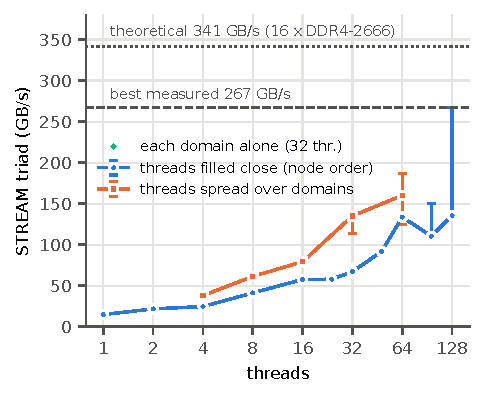
\includegraphics[width=0.6\linewidth]{figures/fig_stream.pdf}
  \caption{STREAM triad bandwidth against thread count (median of 10 runs, bars min--max).}
  \label{fig:stream}
\end{figure}

\subsection{Attainable floating-point performance}
A micro-benchmark of independent fused multiply-add chains on 2-lane NEON registers reaches
4.0 flop/cycle per core, 10.4\GFs{} per core and \textbf{1330\GFs{}} for 128 cores, with perfect scaling.
Scalar FMA reaches the same value (two scalar FMAs per cycle against one vector FMA), so on this
core NEON does not raise the FMA peak: vectorisation saves instructions, not flops per cycle.
Division is much slower, 0.19\GFs{} per core (24.6\GFs{} per node) for vector divides, which matters for
\kernel{viscosity}, \kernel{calc\_dt} and \kernel{pdv}. The ridge point of the node is
$1330/267\approx 5$\,flop/B (0.7\,flop/B for one core).

\subsection{Analytic kernel model}
For every loop nest of the C kernels we counted by hand the 2D arrays that are read and written and the
floating-point operations per cell (+, $-$, $\times$, $/$, $\sqrt{\cdot}$ count as one; MIN, MAX, fabs and
comparisons as zero). Stencil neighbours are assumed to come from the cache, so each array is streamed from
DRAM once per loop nest. Stores that do not read the line first still cost a write-allocate read.
Table~\ref{tab:model} gives the result: 451\,flop and 2186\,B (1688\,B without write-allocate) per cell and time step,
i.e.\ an intensity of 0.21\,flop/B.

\begin{table}[t]
  \centering\small
  \begin{tabular}{lrrrrr}
\toprule
kernel & calls/step & flop/cell & B/cell & B/cell & AI \\
 & & & (no WA) & (with WA) & (flop/B, WA) \\
\midrule
\texttt{ideal\_gas} & 2.1 & 9 & 32 & 48 & 0.19 \\
\texttt{viscosity} & 1 & 40 & 40 & 48 & 0.83 \\
\texttt{calc\_dt} & 1 & 31 & 80 & 88 & 0.35 \\
\texttt{pdv\_predict} & 1 & 33 & 96 & 120 & 0.28 \\
\texttt{pdv\_correct} & 1 & 33 & 112 & 136 & 0.24 \\
\texttt{revert} & 1 & 0 & 32 & 48 & 0.00 \\
\texttt{accelerate} & 1 & 37 & 80 & 96 & 0.39 \\
\texttt{flux\_calc} & 1 & 10 & 64 & 80 & 0.12 \\
\texttt{advec\_cell} & 2 & 45 & 180 & 244 & 0.18 \\
\texttt{advec\_mom} & 4 & 39 & 172 & 220 & 0.18 \\
\texttt{reset\_field} & 1 & 0 & 64 & 96 & 0.00 \\
\texttt{field\_summary} & 0.1 & 22 & 48 & 48 & 0.46 \\
\midrule
per cell and step & & 451 & 1688 & 2186 & 0.21 \\
\bottomrule
\end{tabular}

  \caption{Analytic flop and byte counts per cell (WA = write-allocate). \kernel{ideal\_gas} runs 2.1
    times per step (once more every 10th step).}
  \label{tab:model}
\end{table}

\paragraph{Validation.}
The model predicts 2.80\,TB of DRAM traffic for bm3840. The DDR-controller counters measure 2.83\,TB
(1$\times$128, THP off), 2.87\,TB (4$\times$32) and 2.94\,TB (1$\times$128 default): 1\%, 2\% and 5\%
above the model. The measured read:write ratio of 2.6--2.9 matches the model as well.
The write-allocate version of the model is the right one; this CPU does read lines before overwriting them.
For the pure-copy kernels \kernel{revert} and \kernel{reset\_field} the bus-access counter agrees with the
write-allocate model within 4\% and 35\%. We note that the core-level bus counter overestimates DRAM traffic by
about 1.8$\times$ for stencil kernels because it also counts L3 hits.

\subsection{Roofline of the kernels}
Figure~\ref{fig:roofline} places every kernel on the rooflines of one core and of the full node.
\begin{figure}[t]
  \centering
  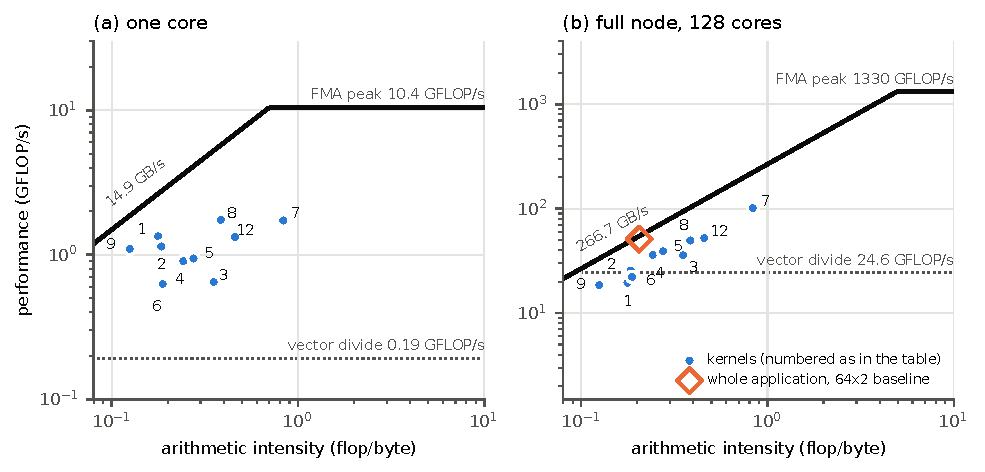
\includegraphics[width=\linewidth]{figures/fig_roofline.pdf}
  \caption{Roofline of the CloverLeaf C kernels (bm3840). Kernel numbers refer to Table~\ref{tab:kernels}.
    Kernel points use analytic bytes and per-kernel PAPI times; the whole-application points use the
    measured DRAM bytes and the median wall clock. The memory ceilings are the STREAM triad values of
    one core and of the full node.}
  \label{fig:roofline}
\end{figure}
The conclusions are:
\begin{itemize}
  \item \textbf{Everything is memory-bound.} All kernels have an intensity of 0.13--0.83\,flop/B, far to the left of
        the node's ridge point (5\,flop/B). Even the most intense kernel, \kernel{viscosity}, would reach only
        222\GFs{} (17\% of the FMA peak) with perfect bandwidth.
  \item \textbf{On one core}, kernels reach 0.6--1.7\GFs{} and 2--9\GBs{}, 12--59\% of the single-core
        bandwidth. The scalar kernels (\kernel{ideal\_gas}, \kernel{calc\_dt}, \kernel{viscosity}) lie
        furthest below the memory roofline; they are limited by instruction latency (divide, square root).
  \item \textbf{On the full node}, the kernels reach 100--150\GBs{} (model bytes) with the default THP
        setting, i.e.\ 38--56\% of the ceiling; the placement problem of Section~\ref{sec:thp} is what keeps
        them below it.
  \item \textbf{Whole application:} the default 1$\times$128 run attains 25\GFs{} (46\% of the 55\GFs{}
        attainable at this intensity), the run with THP disabled 43\GFs{} (\textbf{78\%}), and the 4$\times$32
        run 44\GFs{} (80\%).
  \item \textbf{Floor:} at the measured byte count and the best STREAM bandwidth the 87 steps cannot
        take less than \textbf{10.5\,s}; the best measured time is 13.0\,s. The remaining headroom at the current
        traffic is thus 1.2$\times$; larger gains need fewer bytes.
\end{itemize}

% =============================================================================
\section{From the analysis to optimisations}
\label{sec:opt}
% =============================================================================
The analysis fixes the order of the work: first remove the placement problem (done, 1.7$\times$), then
reduce the number of bytes moved per time step, then the synchronisation overhead. The byte reductions
below are predicted with the analytic model and will be verified with the DDR-controller counters.

\begin{table}[t]
  \centering\small
  \begin{tabular}{llr}
    \toprule
    change & rationale & predicted DRAM bytes \\
    \midrule
    \kernel{advec\_mom}: compute the four direction-only helper arrays once per sweep
      & identical for \texttt{xvel} and \texttt{yvel} & $-13\%$ \\
    \kernel{advec\_cell}: keep four temporaries in registers
      & \kernel{pre\_mass}, \kernel{post\_mass}, \kernel{post\_ener}, \kernel{advec\_vol} & $-6\%$ \\
    drop stores that are never read & \kernel{post\_vol}, \kernel{pre\_vol} & $-4\%$ \\
    \kernel{calc\_dt}: fuse the minimum reduction & \kernel{dt\_min} written and re-read & $-1\%$ \\
    \texttt{nowait} on independent loops & 12.5\% of cycles in barriers & (time only) \\
    \texttt{-fno-math-errno} for the scalar kernels & \texttt{sqrt} blocks vectorisation & (time only) \\
    \bottomrule
  \end{tabular}
  \caption{Planned optimisations and their predicted effect on DRAM traffic (model, with write-allocate).}
  \label{tab:plan}
\end{table}

\todo{M3: implement the changes of Table~\ref{tab:plan} on the 1x128 THP-off baseline, verify each with the
quality check and the DDR counters, report speed-up and the updated roofline.}

% =============================================================================
\section{Conclusions (draft)}
% =============================================================================
\begin{itemize}
  \item CloverLeaf's C kernels are memory-bound on the Kunpeng~920: the whole run has an intensity of
        0.2\,flop/B against a ridge point of 5\,flop/B. Compute-side optimisation cannot pay off.
  \item The analytic traffic model is accurate to 1--5\% of the measured DRAM traffic and can therefore be
        used to predict the effect of optimisations.
  \item The largest single inefficiency of the baseline was not in the kernels but in memory placement:
        transparent huge pages unbalance the NUMA domains and cost a factor 1.7 in pure-OpenMP runs.
  \item At the current traffic the code is within 1.2$\times$ of the memory-bound floor; further speed-up
        has to come from moving fewer bytes and from fewer barriers.
\end{itemize}

\bibliographystyle{plain}
\bibliography{refs}

\end{document}
